\section{Introducción \label{sec:cap_three_introduction}}
El presente capítulo se encuentra orientado a la explicación de los objetivos detectados,de cómo las metodologías escogidas en el área de Ingeniería de Software y Descubrimiento del Conocimiento son utilizadas en el desarrollo de la solución y finalmente una descripción de los requerimientos levantados así como la descripción de los datos a utilizar para la realización de las estimaciones de demanda.

\section{Objetivos \label{sec:goals}}

Frente a la necesidad presentada de poder gestionar de forma adecuada la planificación de cursos y profesores dentro de la Escuela de Ingeniería en el contexto del nuevo curriculum, se identifica como objetivo principal calcular la cantidad de alumnos para un curso específico en el siguiente periodo académico, es decir, calcular la demanda para un curso en el siguiente semestre académico. Este objetivo plantea una serie de objetivos secundarios necesarios para el cumplimiento de éste. A continuación se enuncian estos objetivos secundarios para un mejor entendimiento del contexto en el cual se desenvuelve la problemática:

\section{Subsistemas y Metodología de Trabajo \label{sec:work_environment}}

\begin{enumerate}
	\item \textbf{Objetivo Principal:} Predecir en forma aproximada la demanda de alumnos para un curso específico en el siguiente semestre.
	\item \textbf{Objetivos Secundarios}
		\begin{enumerate}
			\item Tener una representación de la estructura de unidades académicas de la universidad en cada uno de sus niveles: escuelas e institutos.
			\item Apoyar en la gestión de los cursos del primer ciclo formativo (Licenciatura),  distribuidos en sus componentes básicas: plan de ciencias básicas, major y minor.
			\item Apoyar en la gestión de los majors y minors existentes así como la relación entre ellos.
			\item Apoyar en la gestión de cursos en las unidades académicas.
			\item Manejar la información histórica correspondiente al avance curricular por alumno en cada una de las generaciones.
			\item Evaluar diferentes estrategias de entrenamiento y predicción en los análisis predictivos de modo de  tener modelos actualizados.
			\item Visualizar las estimaciones históricas realizadas en base a la información que se posee.
		\end{enumerate}
\end{enumerate}

\subsection{Subsistemas \label{sec:sub_systems}}
Los objetivos planteados son respondidos mediante 3 grandes subsistemas:  una plataforma web que permite el almacenamiento de la información de histórica de los alumnos,  un conjunto de módulos para la creación de modelos predictivos y ua módulo de reportería que permite comparar los resultados para un curso en particular. La figura \ref{fig:subsystems} muestra los objetivos asociados a cada uno de estos subsistemas.

\begin{figure}[ht]
	\begin{center}
	  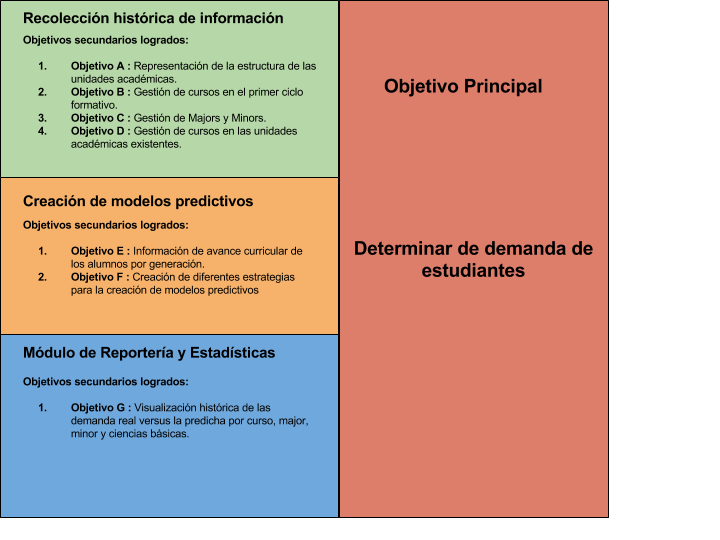
\includegraphics[width=0.8\textwidth]{./figures/chapter_03/01_objetivos.png}
	  \setcaptioncitation{Fuente Propia}
	  \caption{Subsistemas y sus objetivos}
	  \label{fig:subsystems}
	\end{center}
\end{figure}

\subsection{Metodología de trabajo \label{sec:work_methodology}}

La primera etapa incluye, por un lado, un levantamiento de los requerimientos funcionales, y por otro el análisis y preparación de los datos y utilizamos para ello métodos asociados a \textit{Extreme Programming (XP)} y \textit{Adaptive Software Development-Data Mining (ASD-DM)} respectivamente.   Los requerimientos funcionales quedan sintetizados en forma de relatos de usuario asociados a un conjunto de épicas.

Luego de la etapa inicial descrita anteriormente, se da inicio al proceso de desarrollo de software propiamente tal en forma iterativa e incremental, es decir, la creación sucesiva de pequeños entregables acumulativos usando un proceso iterativo de conversaciones con los \textit{stakeholders}. En paralelo con ello se lleva a cabo el proceso cíclico de modelación y evaluación de los algoritmos predictivos en \textit{ASDM-DM}.

\section{Requisitos \label{sec:requirements}}
\subsection{Usuarios \label{sec:user_description}}

La plataforma posee los siguientes tipos de usuarios o roles:

\begin{enumerate}
	\item \textbf{Administrador:} Manejo de usuarios, modelos predictivos, ejecuciones de entrenamiento y predicción, informes.
	\item \textbf{Estadístico:} Rol encargado de la mejora de los modelos estadístico, para ello puede solicitar entrenar modelos con diferentes estrategias y carga de modelos DSF en el sistema para un curso en particular. También posee la opción de realizar diferentes predicciones en un curso en particular o de todos los cursos cargados en el sistema.
	\item \textbf{Analista:} Puede correr nuevas predicciones y ver los resultados relativos a esas predicciones. Al mismo tiempo, puede ver la información acerca de los majors, minors, estudiantes y la historia de los mismos.
\end{enumerate}

\subsection{Épicas \label{sec:user_description}}

Las épicas corresponden a grupos de relatos de usuario que en forma conjunta permiten constituir una funcionalidad mayor. La siguiente lista muestra las épicas identificadas en este proyecto:

\begin{enumerate}
	\item \textbf{Administrador de Majors:} Permite la gestión de los majors dentro de la aplicación, es decir, la creación, eliminación , edición y la visualización dentro de la solución a implementarse. Adicionalmente, provee la posibilidad de administrar los cursos pertenecientes a cada major en particular.
	\item \textbf{Administrador de Minors:} Permite la gestión de los minors dentro de la aplicación, es decir, la creación, eliminación , edición y la visualización dentro de la solución a implementarse. Adicionalmente, provee la posibilidad de administrar los cursos pertenecientes a cada major en particular.
	\item \textbf{Carga de alumnos:} Corresponde a todas las funcionales que permiten la carga de información demográfica y de la universidad del alumno, tales como declaraciones de majors, minors, edad, generación, entre otras.
	\item \textbf{Carga de cursos:} Otorga la posibilidad de subir la información de los cursos y requisitos a través de un módulo de carga vía excel.
	\item \textbf{Carga de información histórica de un alumno:} Es el módulo encargado de validar y permite subir el avance curricular de los alumnos al sistema vía un archivo excel. Además, entrega indica cuando alguna información no entrega el formato esperado por el sistema.
	\item \textbf{Validar información de los cursos:} Conjunto de funcionalidades que permiten establecer el formato adecuado para la carga de los cursos de la universidad por unidad académica. Además, debe indicar el campo o los campos que no cumplen con el formato exigido.
	\item \textbf{Validar información de alumno:} Conjunto de funcionalidades que permiten establecer el formato adecuado para la carga de los alumnos. Además, debe indicar el campo o los campos que no cumplen con el formato exigido.
	\item \textbf{Validar información histórica de un alumno:} Conjunto de funcionalidades que permiten establecer el formato adecuado para el avance curricular de los alumnos. Además, debe indicar el campo o los campos que no cumplen con el formato exigido.
	\item \textbf{Laboratorio Predictivo:} Es la infraestructura y conjunto de funcionalidad que permite ejecutar modelos en el lenguaje de programación R, cuyos resultados son almacenados en la base de datos que utiliza el sistema.
	\item \textbf{Laboratorio de Entrenamiento:} Permite definir estrategias de entrenamiento sobre los datos históricos de los alumnos con el objetivo de poder mejorar la precisión de los modelos. Además, permite la gestión y almacenamiento de modelos en el formato RDS y \textit{scritps} \dictionary{script} del lenguaje R para la ejecución de modelos.
	\item \textbf{Otro:} Agrupa a todos aquellos relatos de usuarios que no encuentran en un epic anterior. Abarcan diferentes objetivos del software y ,por lo mismo, los relatos de usuarios no necesariamente presentan una correlación entre ellos.
\end{enumerate}

\subsection{Relatos de usuarios agrupados por Épicas \label{sec:detailed_user_stories}}

\subsubsection{Administrador de Majors}

\begin{enumerate}
	\item Relato 01
		\begin{enumerate}
			\item \textbf{Descripción:} Como administrador deseo desde el menú superior poder acceder a la opción Majors, así poder visualizar los majors creados en el sistema.
			\item \textbf{Criterios de aceptación}
				\begin{enumerate}
					\item Dado que ingresé a la sección Majors, el sistema me muestra una tabla paginada de los majors existentes en el sistema ordenados por fecha de creación. Los campos de la tabla corresponde a: nombre major y departamento al cual pertenecen.
					\item Dado que estoy la tabla paginada de los majors existentes, desde uno en particular es posible acceder al detalle de un major, eliminarlo. Al realizar la eliminación se elimina el major y las asociaciones respectivas con los cursos, sin eliminar estos últimos.
					\item Desde la tabla paginada, en la parte superior derecha existe un nuevo botón indicando \textbf{Nuevo Major}. El sistema despliega un formulario solicitando nombre y departamentos encargados.
				\end{enumerate}
		\end{enumerate}
	\item Relato 02
		\begin{enumerate}
			\item \textbf{Descripción:} Como un Administrador deseo poder visualizar el detalle de un major, el cual incluye un listado de cursos asociados al major indicando qué cursos son obligatorios y opcionales, así puedo visualizar el listado completo de cursos.
			\item \textbf{Criterios de aceptación}
				\begin{enumerate}
					\item Dado que ingresé al detalle de un major, la tabla paginada me muestra la sigla del curso, nombre,nombre del departamento cual lo dicta e indicando si el curso es obligatorio u opcional.
				\end{enumerate}
		\end{enumerate}
	\item Relato 03
		\begin{enumerate}
			\item \textbf{Descripción:} Como un Administrador deseo poder incorporar un nuevo curso a un major disponible en el sistema, así puedo administrar la estructura de los majors.
			\item \textbf{Criterios de aceptación}
				\begin{enumerate}
					\item Dado que estoy visualizando la tabla de cursos en el major, el sistema en la parte superior derecha de la tabla se podrá visualizar un botón que indica \textbf{Agregar Curso}.
					\item Dado incorporé un curso ya existente en la estructura, el sistema debe rechazar la incorporación de este.
				\end{enumerate}
		\end{enumerate}
	\item Relato 04
		\begin{enumerate}
			\item \textbf{Descripción:} Como un Estadístico deseo desde el menú superior poder acceder a la opción Majors, así poder visualizar los majors creados en el sistema.
			\item \textbf{Criterios de aceptación}
				\begin{enumerate}
					\item Dado que ingresé a la sección Majors, el sistema me muestra una tabla paginada de los majors existentes en el sistema ordenados por fecha de creación. Los campos de la tabla corresponde a: nombre major y departamento al cual pertenecen.
					\item Dado que estoy la tabla paginada de los majors existentes, desde uno en particular es posible acceder al detalle de un major, eliminarlo. Al realizar la eliminación se elimina el major y las asociaciones respectivas con los cursos, sin eliminar estos últimos.
				\end{enumerate}
		\end{enumerate}
	\item Relato 05
		\begin{enumerate}
			\item \textbf{Descripción:} Como un Estadístico deseo poder visualizar el detalle de un major, el cual incluye un listado de cursos asociados al major indicando qué cursos son obligatorios y opcionales, así puedo visualizar el listado completo de cursos.
			\item \textbf{Criterios de aceptación}
				\begin{enumerate}
					\item Dado que ingresé al detalle de un major, la tabla paginada me muestra la sigla del curso, nombre, nombre del departamento cual lo dicta e indicando si el curso es obligatorio u opcional.
				\end{enumerate}
		\end{enumerate}
	\item Relato 06
		\begin{enumerate}
			\item \textbf{Descripción:} Como un Estadístico deseo poder incorporar un nuevo curso a un major disponible en el sistema, así puedo administrar la estructura de los majors.
			\item \textbf{Criterios de aceptación}
				\begin{enumerate}
					\item Dado que estoy visualizando la tabla de cursos en el major, el sistema en la parte superior derecha de la tabla se podrá visualizar un botón que indica \textbf{Agregar Curso}.
					\item Dado incorporé un curso ya existente en la estructura, el sistema debe rechazar la incorporación de este.
				\end{enumerate}
		\end{enumerate}
\end{enumerate}

\subsubsection{Administrador de Minors}

\begin{enumerate}
	\item Relato 01
		\begin{enumerate}
			\item \textbf{Descripción:} Como un Administrador deseo desde el menú superior poder acceder a la opción Minors, así puedo reorganizar nuevos elementos dentro del minor.
			\item \textbf{Criterios de aceptación}
				\begin{enumerate}
					\item Dado que accedí a la opción Minors, se muestra una tabla pagina de los minors en el sistema, indicando nombre, fecha de creación y departamentos/facultades participantes en esté.
				\end{enumerate}
		\end{enumerate}
	\item Relato 02
		\begin{enumerate}
			\item \textbf{Descripción:} Como un Administrador deseo poder incorporar un nuevo curso a un minor disponible en el sistema, así puedo identificar el nivel de importancia del minor dentro de los estudiantes.
			\item \textbf{Criterios de aceptación}
				\begin{enumerate}
					\item Dado que estoy visualizando la lista de minors, en la parte superior derecha existe un botón que indica \textbf{Nuevo Minor}, al presionarlo se abre otra ventana con los datos en la tabla.
					\item Dado que estoy en el formulario de incorporación de cursos al minor, el curso debe existir previamente en el sistema. No es posible crearlo desde esta ventana.
					\item Dado que estoy en un formulario de asociación, el sistema debe consultar si el curso dentro del minor es optativo u obligatorio.
				\end{enumerate}
		\end{enumerate}
	\item Relato 03
		\begin{enumerate}
			\item \textbf{Descripción:} Como un Administrador deseo poder visualizar la estructura de cursos y alumnos han inscrito el minor, así puedo visualizar la cantidad total de minors en el sistema.
			\item \textbf{Criterios de aceptación}
				\begin{enumerate}
					\item Dado que estoy en la lista de minor disponibles en el sistema, en una columna existe una opción denominada \textbf{Ver detalle}, al hacer click en ella, el sistema me lleva a otra ventana donde se detalle una lista de los cursos pertenecientes al minor, alumnos que hay inscritos en él y un botón que indica \textbf{Incorporar curso}.
					\item Dado que estoy en la lista de cursos disponibles en el minor, al lado de cada curso existen las opciones de \textbf{desvincular} y cambiar estado de obligatorio a opcional y viceversa.
				\end{enumerate}
		\end{enumerate}
	\item Relato 04
		\begin{enumerate}
			\item \textbf{Descripción:} Como un Estadístico deseo desde el menú superior poder acceder a la opción Minors, así puedo reorganizar nuevos elementos dentro del minor.
			\item \textbf{Criterios de aceptación}
				\begin{enumerate}
					\item Dado que accedí a la opción Minors, se muestra una tabla página de los minors en el sistema, indicando nombre, fecha de creación y departamentos/facultades participantes en este.
				\end{enumerate}
		\end{enumerate}
	\item Relato 05
		\begin{enumerate}
			\item \textbf{Descripción:} Como un Estadístico deseo poder incorporar un nuevo curso a un minor disponible en el sistema, así puedo identificar el nivel de importancia del minor dentro de los estudiantes.
			\item \textbf{Criterios de aceptación}
				\begin{enumerate}
					\item Dado que estoy visualizando la lista de minors, en la parte superior derecha existe un botón que indica \textbf{Nuevo Minor}, al presionarlo se abre otra ventana con los datos en la tabla.
					\item Dado que estoy en el formulario de incorporación de cursos al minor, el curso debe existir previamente en el sistema. No es posible crearlo desde esta ventana.
					\item Dado que estoy en un formulario de asociación, el sistema debe consultar si el curso dentro del minor es optativo u obligatorio.
				\end{enumerate}
		\end{enumerate}
	\item Relato 06
		\begin{enumerate}
			\item \textbf{Descripción:} Como un Estadístico deseo poder visualizar la estructura de cursos y alumnos han inscrito el minor, así puedo mantener actualizado la información de los alumnos en el sistema.
			\item \textbf{Criterios de aceptación}
				\begin{enumerate}
					\item Dado que estoy en la lista de minor disponibles en el sistema, en una columna existe una opción denominada \textbf{Ver detalle}, al hacer click en ella, el sistema me lleva a otra ventana donde se detalle una lista de los cursos pertenecientes al minor, alumnos que hay inscritos en él y un botón que indica \textbf{"Incorporar curso"}.
					\item Dado que estoy en la lista de cursos disponibles en el minor, al lado de cada curso existen las opciones de \textbf{desvincular} y cambiar estado de obligatorio a opcional y viceversa.
				\end{enumerate}
		\end{enumerate}
\end{enumerate}

\subsubsection{Carga de alumnos}

\begin{enumerate}
	\item Relato 01
		\begin{enumerate}
			\item \textbf{Descripción:} Como un Administrador deseo poder carga un archivo excel con nuevos alumnos, así puedo ingresar nueva información histórica de alumnos
			\item \textbf{Criterios de aceptación}
				\begin{enumerate}
					\item Dado que ingresé a la sección alumnos, el sistema me muestra un formulario con la opción de de subir un archivo excel.
					\item Dado que visualicé el formulario para subir archivos, debajo de él existe una plantilla excel indicando los elementos y formato que se requieren. Los campos solicitados son rut, nombre, apellido paterno, apellido materno, generación, declaración de major a través de su código, declaración de minors a través de su código, major escogido a través de su código y minor a través de su código.
				\end{enumerate}
		\end{enumerate}
	\item Relato 02
		\begin{enumerate}
			\item \textbf{Descripción:} Como un Estadístico deseo poder carga un archivo excel con nuevos alumnos, así puedo ingresar nueva información histórica de alumnos.
			\item \textbf{Criterios de aceptación}
				\begin{enumerate}
					\item Dado que ingresé a la sección alumnos, el sistema me muestra un formulario con la opción de de subir un archivo excel.
					\item Dado que visualicé el formulario para subir archivos, debajo de él existe una plantilla excel indicando los elementos y formato que se requieren. Los campos solicitados son rut, nombre, apellido paterno, apellido materno, generación, declaración de major a través de su código, declaración de minors a través de su código, major escogido a través de su código y minor a través de su código.
				\end{enumerate}
		\end{enumerate}
	\item Relato 03
		\begin{enumerate}
			\item \textbf{Descripción:} Como un Analista deseo poder carga un archivo excel con nuevos alumnos, así puedo ingresar nueva información histórica de alumnos.
			\item \textbf{Criterios de aceptación}
				\begin{enumerate}
					\item Dado que ingresé a la sección alumnos, el sistema me muestra un formulario con la opción de de subir un archivo excel.
					\item Dado que visualicé el formulario para subir archivos, debajo de él existe una plantilla excel indicando los elementos y formato que se requieren. Los campos solicitados son rut, nombre, apellido paterno, apellido materno, generación, declaración de major a través de su código, declaración de minors a través de su código, major escogido a través de su código y minor a través de su código.
				\end{enumerate}
		\end{enumerate}
	\item Relato 04
		\begin{enumerate}
			\item \textbf{Descripción:} Como un Administrador deseo poder revisar las cargas de alumnos que se han realizado, así puedo llevar un control de los alumnos que se han ingresado al sistema.
			\item \textbf{Criterios de aceptación}
				\begin{enumerate}
					\item Dado que estoy en la página inicial, desde el menú Alumnos es posible obtener una opción para acceder a la cargas realizadas.
					\item Dado que hice click en la opción de cargas realizadas, el sistema me muestra una tabla paginada con el responsable, cantidad de alumnos y fecha de realización de la carga.
					\item Dado que ingresé al detalle de una carga, es posible tener la opción de eliminar la información de los alumnos subidos. Se borra toda la información relacionada, historial de cursos, predicciones realizadas.
				\end{enumerate}
		\end{enumerate}
	\item Relato 05
		\begin{enumerate}
			\item \textbf{Descripción:} Como un Estadístico deseo poder revisar las cargas de alumnos que se han realizado, así puedo llevar un control de los alumnos que se han ingresado al sistema.
			\item \textbf{Criterios de aceptación}
				\begin{enumerate}
					\item Dado que estoy en la página inicial, desde el menú Alumnos es posible obtener una opción para acceder a la cargas realizadas.
					\item Dado que hice click en la opción de cargas realizadas, el sistema me muestra una tabla paginada con el responsable, cantidad de alumnos y fecha de realización de la carga.
				\end{enumerate}
		\end{enumerate}
\end{enumerate}

\subsubsection{Carga de cursos}

\begin{enumerate}
	\item Relato 01
		\begin{enumerate}
			\item \textbf{Descripción:} Como un Administrador deseo poder cargar cursos a través de un archivo excel, así puedo ingresarlos al momento de que se creen en la UC.
			\item \textbf{Criterios de Aceptación}
				\begin{enumerate}
					\item Dado que me encuentro en la sección cursos, arriba de la tabla existe un formulario para ingresar un nuevo archivo excel.
					\item Dado que me encuentro en la sección cursos, debajo del formulario para subir nuevos cursos puedo descargar un archivo excel de plantilla para cumplir el formato requerido.
					\item Dado que ingresé un formulario completo, con datos correctos e hice click en el botón Cargar Cursos, en caso de que cumplan el formato, el sistema debe entregar un mensaje de éxito.
				\end{enumerate}
		\end{enumerate}
	\item Relato 02
		\begin{enumerate}
			\item \textbf{Descripción:} Como un Estadístico deseo poder cargar cursos a través de un archivo excel, asi puedo ingresarlos al momento de que se creen en la UC.
			\item \textbf{Criterios de Aceptación}
				\begin{enumerate}
					\item Dado que me encuentro en la sección cursos, arriba de la tabla existe un formulario para ingresar un nuevo archivo excel.
					\item Dado que me encuentro en la sección cursos, debajo del formulario para subir nuevos cursos puedo descargar un archivo excel de plantilla para cumplir el formato requerido.
					\item Dado que ingresé un formulario completo, con datos correctos e hice click en el botón Cargar Cursos, en caso de que cumplan el formato, el sistema debe entregar un mensaje de éxito.
				\end{enumerate}
		\end{enumerate}
	\item Relato 03
		\begin{enumerate}
			\item \textbf{Descripción:} Como un Analista deseo poder cargar cursos a través de un archivo excel, asi puedo ingresarlos al momento de que se creen en la UC.
			\item \textbf{Criterios de Aceptación}
				\begin{enumerate}
					\item Dado que me encuentro en la sección cursos, arriba de la tabla existe un formulario para ingresar un nuevo archivo excel.
					\item Dado que me encuentro en la sección cursos, debajo del formulario para subir nuevos cursos puedo descargar un archivo excel de plantilla para cumplir el formato requerido.
					\item Dado que ingresé un formulario completo, con datos correctos e hice click en el botón Cargar Cursos, en caso de que cumplan el formato, el sistema debe entregar un mensaje de éxito.
				\end{enumerate}
		\end{enumerate}
	\item Relato 04
		\begin{enumerate}
			\item \textbf{Descripción:} Como un Administrador deseo poder revisar la cargas que he realizado, así puedo llevar un seguimiento de qué cursos y cuándo se han cargado.
			\item \textbf{Criterios de Aceptación}
				\begin{enumerate}
					\item Desde el menú superior Cursos, el sistema me muestra la opción de acceder a historial de cargas.
					\item Dado que accedí al historial de descargar, el sistema me indica una tabla paginada indicando fecha de la carga de cursos, cantidad de cursos cargados y la opción para ver el detalle.
				\end{enumerate}
		\end{enumerate}
	\item Relato 05
		\begin{enumerate}
			\item \textbf{Descripción:} Como un Administrador deseo poder visualizar el detalle de una carga histórica, así puedo revisar de modo específico qué cursos se cargaron y quién fue el usuario que lo realizó.
			\item \textbf{Criterios de Aceptación}
				\begin{enumerate}
					\item Dado que presioné un click sobre la opción visualizar detalle desde la tabla página de historial de carga, el sistema me indica de modo general el usuario que realizó la carga, la cantidad de cursos cargados, la fecha de carga y una tabla paginada indicando los cursos subidos.
				\end{enumerate}
		\end{enumerate}
\end{enumerate}

\subsubsection{Carga de información histórica de un alumno}

\begin{enumerate}
	\item Relato 01
		\begin{enumerate}
			\item \textbf{Descripción:} Como un Administrador deseo poder información histórica de rendimiento de uno o varios a alumnos a través de un archivo excel, así puedo estar seguro de que el sistema usa la misma nomenclatura para la información histórica de alumnos.
			\item \textbf{Criterios de aceptación}
				\begin{enumerate}
					\item Dado que me encuentro en la lista de alumnos disponibles en el sistema, desde un lugar entre el menú superior y la tabla de los alumnos, exista un formulario donde se me da la opción de subir el archivo excel.
					\item Dado que estoy visualizando el formulario para el archivo excel, existe un link de descarga con la plantilla que puedo seguir. En ella se me indican los campos y formatos que debo seguir.
				\end{enumerate}
		\end{enumerate}
	\item Relato 02
		\begin{enumerate}
			\item \textbf{Descripción:} Como un Estadístico poder cargar la información histórica de rendimiento de uno o varios a alumnos a través de un archivo excel, así puedo estar seguro de que el sistema usa la misma nomenclatura para la información histórica de alumnos.
			\item \textbf{Criterios de aceptación}
				\begin{enumerate}
					\item Dado que me encuentro en la lista de alumnos disponibles en el sistema, desde un lugar entre el menú superior y la tabla de los alumnos, exista un formulario donde se me da la opción de subir el archivo excel.
					\item Dado que estoy visualizando el formulario para el archivo excel, existe un link de descarga con la plantilla que puedo seguir. En ella se me indican los campos y formatos que debo seguir.
				\end{enumerate}
		\end{enumerate}
	\item Relato 03
		\begin{enumerate}
			\item \textbf{Descripción:} Como un Analista deseo poder información histórica de rendimiento de uno o varios a alumnos a través de un archivo excel, así puedo estar seguro de que el sistema usa la misma nomenclatura para la información histórica de alumnos.
			\item \textbf{Criterios de aceptación}
				\begin{enumerate}
					\item Dado que me encuentro en la lista de alumnos disponibles en el sistema, desde un lugar entre el menú superior y la tabla de los alumnos, exista un formulario donde se me da la opción de subir el archivo excel.
					\item Dado que estoy visualizando el formulario para el archivo excel, existe un link de descarga con la plantilla que puedo seguir. En ella se me indican los campos y formatos que debo seguir.
				\end{enumerate}
		\end{enumerate}
\end{enumerate}

\subsubsection{Validar información de los cursos}

\begin{enumerate}
	\item Relato 01
		\begin{enumerate}
			\item \textbf{Descripción:} Como un Administrador deseo recibir un email cuando los cursos hayan sido validados y cargados en el sistema, así puedo asegurarme que la información cargada tenga la misma nomenclatura
			\item \textbf{Criterios de aceptación}
				\begin{enumerate}
					\item Dado que ingresé un excel al formulario con datos incorrectos, el sistema me debe indicar la línea y columna que no cumple con el formato requerido.
					\item Dado que ingresé un sigla ya existente, el sistema debe indicarme que no es posible crear este curso indicando fila y sigla existente.
					\item Dado que el ingresé una sigla, el nombre no puede estar vacío.
				\end{enumerate}
		\end{enumerate}
	\item Relato 02
		\begin{enumerate}
			\item \textbf{Descripción:} Como un Estadístico deseo recibir un email cuando los cursos hayan sido validados y cargados en el sistema, así puedo asegurarme que la información cargada tenga la misma nomenclatura
			\item \textbf{Criterios de aceptación}
				\begin{enumerate}
					\item Dado que ingresé un excel al formulario con datos incorrectos, el sistema me debe indicar la línea y columna que no cumple con el formato requerido.
					\item Dado que ingresé un sigla ya existente, el sistema debe indicarme que no es posible crear este curso indicando fila y sigla existente.
					\item Dado que el ingresé una sigla, el nombre no puede estar vacío.
				\end{enumerate}
		\end{enumerate}
	\item Relato 03
		\begin{enumerate}
			\item \textbf{Descripción:} Como un Analista deseo recibir un email cuando los cursos hayan sido validados y cargados en el sistema, así puedo asegurarme que la información cargada tenga la misma nomenclatura.
			\item \textbf{Criterios de aceptación}
				\begin{enumerate}
					\item Dado que ingresé un excel al formulario con datos incorrectos, el sistema me debe indicar la línea y columna que no cumple con el formato requerido.
					\item Dado que ingresé un sigla ya existente, el sistema debe indicarme que no es posible crear este curso indicando fila y sigla existente.
					\item Dado que el ingresé una sigla, el nombre no puede estar vacío.
				\end{enumerate}
		\end{enumerate}
\end{enumerate}

\subsubsection{Validar información de alumno}

\begin{enumerate}
	\item Relato 01
		\begin{enumerate}
			\item \textbf{Descripción:} Como un Administrador deseo poder recibir el resultado de la carga de nuevos alumnos vía email y en la pantalla del usuario, así verificar que se use la misma nomenclatura para todos los participantes del sistema.
			\item \textbf{Criterios de Aceptación:}
				\begin{enumerate}
					\item Dado que ingresé un archivo excel con información correcta, el sistema me indica un mensaje de éxito.
					\item Dado que ingresé un archivo excel con información incorrecta en formato, el sistema me indica la fila y columna e indicando que existe un error de formato. Además, indica cómo el campo debe ser completado.
					\item Dado que ingresé un archivo excel con información ya existente, el sistema me indica la fila y columna e indica cuál es la información duplicada.
				\end{enumerate}
		\end{enumerate}
	\item Relato 02
		\begin{enumerate}
			\item \textbf{Descripción:} Como un Estadístico deseo poder recibir el resultado de la carga de nuevos alumnos vía email y en la pantalla del usuario, así verificar que se use la misma nomenclatura para todos los participantes del sistema.
			\item \textbf{Criterios de Aceptación:}
				\begin{enumerate}
					\item Dado que ingresé un archivo excel con información correcta, el sistema me indica un mensaje de éxito.
					\item Dado que ingresé un archivo excel con información incorrecta en formato, el sistema me indica la fila y columna e indicando que existe un error de formato. Además, indica cómo el campo debe ser completado.
					\item Dado que ingresé un archivo excel con información ya existente, el sistema me indica la fila y columna e indica cuál es la información duplicada.
				\end{enumerate}
		\end{enumerate}
	\item Relato 03
		\begin{enumerate}
			\item \textbf{Descripción:} Como un Analista deseo poder recibir el resultado de la carga de nuevos alumnos vía email y en la pantalla del usuario, así verificar que se use la misma nomenclatura para todos los participantes del sistema.
			\item \textbf{Criterios de Aceptación:}
				\begin{enumerate}
					\item Dado que ingresé un archivo excel con información correcta, el sistema me indica un mensaje de éxito.
					\item Dado que ingresé un archivo excel con información incorrecta en formato, el sistema me indica la fila y columna e indicando que existe un error de formato. Además, indica cómo el campo debe ser completado.
					\item Dado que ingresé un archivo excel con información ya existente, el sistema me indica la fila y columna e indica cuál es la información duplicada.
				\end{enumerate}
		\end{enumerate}
\end{enumerate}

\subsubsection{Validar información histórica de un alumno}

\begin{enumerate}
	\item Relato 01
		\begin{enumerate}
			\item \textbf{Descripción:} Como un Administrador deseo poder saber que la información que incorporé en el excel se haya subido de forma exitosa, así puedo saber si se mantiene actualizada.
			\item \textbf{Criterios de Aceptación}
				\begin{enumerate}
					\item Dado que subí un excel con información correcta, el sistema me debe indicar los elementos fueron subidos de forma exitosa.
					\item Dado que subí un excel con información incorrecta, el archivo me debe indicar fila y columna del error, además indicar el tipo de error que existe. Pueden ser por formato o información ya existente.
				\end{enumerate}
		\end{enumerate}
	\item Relato 02
		\begin{enumerate}
			\item \textbf{Descripción:} Como un Estadístico deseo poder saber que la información que incorporé en el excel se haya subido de forma exitosa, así puedo saber si se mantiene actualizada.
			\item \textbf{Criterios de Aceptación}
				\begin{enumerate}
					\item Dado que subí un excel con información correcta, el sistema me debe indicar los elementos fueron subidos de forma exitosa.
					\item Dado que subí un excel con información incorrecta, el archivo me debe indicar fila y columna del error, además indicar el tipo de error que existe. Pueden ser por formato o información ya existente.
				\end{enumerate}
		\end{enumerate}
	\item Relato 03
		\begin{enumerate}
			\item \textbf{Descripción:} Como un Analista deseo poder saber que la información que incorporé en el excel se haya subido de forma exitosa, así puedo saber si se mantiene actualizada.
			\item \textbf{Criterios de Aceptación}
				\begin{enumerate}
					\item Dado que subí un excel con información correcta, el sistema me debe indicar los elementos fueron subidos de forma existosa.
					\item Dado que subí un excel con información incorrecta, el archivo me debe indicar fila y columna del error, además indicar el tipo de error que existe. Pueden ser por formato o información ya existente.
				\end{enumerate}
		\end{enumerate}
\end{enumerate}

\subsubsection{Laboratorio Predictivo}

\begin{enumerate}
	\item Relato 01
		\begin{enumerate}
			\item \textbf{Descripción:} Como un Administrador poder visualizar todos las predicciones realizadas en el sistema según tipo de predicción : curso, major,minor , departamento o conjunto de cursos., así puedo realizar análisis de modo granularidad por los tipo de predicciones realizadas.
			\item \textbf{Criterios de Aceptación}
				\begin{enumerate}
					\item Dado que inicié sesión, puedo visualizar un menú superior denominado Laboratorios y como submenú \textbf{Laboratorio predictivo}.
					\item Dado que hice click en la opción de \textbf{Laboratorio predictivo}, el sistema me dirige la página de las predicciones que se muestran en una tabla paginada indicando  nombre de la predicción, fecha de realización, tipo y botón de acciones. Las opciones son ver detalle y eliminar.
					\item Dado que hice click en eliminar, el sistema debe consultar si estoy seguro de querer realizarla. En caso de aceptar, se borra las predicciones realizadas y no los cursos y asociaciones entre alumnos.
				\end{enumerate}
		\end{enumerate}
	\item Relato 02
		\begin{enumerate}
			\item \textbf{Descripción:} Como un Administrador crear una nueva predicción indicando su nombre, tipo de predicción (curso, major, minor, departamento o conjunto de cursos), así puedo conocer un orden de magnitud de la cantidad de alumnos que tendrá el curso.
			\item \textbf{Criterios de Aceptación}
				\begin{enumerate}
					\item Dado que seleccioné tipo de evaluación curso, puedo seleccionar un curso en específico a través de un select.
					\item Dado que seleccioné tipo de evaluación major o minor, el sistema carga una lista de forma automática de los cursos de los cuales se hará una predicción.
					\item Dado que seleccioné tipo de evaluación departamento, el sistema carga de forma automática la lista de cursos que dicta el departamento.
				\end{enumerate}
		\end{enumerate}
	\item Relato 03
		\begin{enumerate}
			\item \textbf{Descripción:} Como un Administrador poder visualizar el resultado de la predicción por cursos al hacer click en \textbf{detalle} desde la tabla de predicciones realizadas, así puedo realizar visualizar si puedo realizar una predicción de forma correcta por tipo de predicción (curso, major, minor, departamento o conjunto de cursos).
			\item \textbf{Criterios de Aceptación}
				\begin{enumerate}
					\item Dado que realicé la predicción, los detalles esperado son : cantidad de alumnos por curso. En caso de existir más de un curso, se espera tener una tabla paginada ordenada por sigla de cada uno.
				\end{enumerate}
		\end{enumerate}
\end{enumerate}

\subsubsection{Laboratorio de Entrenamiento}

\begin{enumerate}
	\item Relato 01
		\begin{enumerate}
			\item \textbf{Descripción:} Como un Administrador poder visualizar todos los cursos que tienen asignado un modelo predictivo , así poder visualizar si el curso está listo para poder realizar un predicción de la cantidad de alumnos a tomar el próximo semestre.
			\item \textbf{Criterios de Aceptación}
				\begin{enumerate}
					\item Dado que inicié sesión, en la barra superior puedo acceder al menú \textbf{Laboratorio} y como submenu \textbf{Laboratorio de entrenamiento}.
					\item Dado que hice click en la opción \textbf{Laboratorio de entrenamiento}, puedo visualizar una lista de cursos en una tabla con el siguiente detalle : Sigla del curso, nombre del curso, estado (indica si posee  o no un modelo predictivo cargado) y acciones, indicando ver detalle, cargar modelo, carga script de ejecución, carga script de entrenamiento y eliminar. (Los script cargados deben ser en código R).
					\item Dado que seleccioné la opción eliminar, el sistema me indica un mensaje indicando si estoy seguro de hacerlo. En caso afirmativo, el sistema borra el script de ejecución del modelo junto al modelo cargado.
				\end{enumerate}
		\end{enumerate}
	\item Relato 02
		\begin{enumerate}
			\item \textbf{Descripción:} Como un Administrador poder visualizar el detalle de un curso en el laboratorio predictivo, así puedo estar seguro de que mi modelo se está entrenando con una buena calidad.
			\item \textbf{Criterios de Aceptación}
				\begin{enumerate}
					\item Dado que hice click en la parte \textbf{detalle} de la lista de cursos en el laboratorio predictivo, el sistema me lleva a una página indicando sigla, nombre y departamento que lo dicta (en caso de ser un curso en conjunto, se muestra la lista de los departamentos), checklist de scripts cargados o creados para el o los cursos indicando si el script de predicción, entrenamiento y modelo se encuentran creados.
					\item Dado que me encuentro en el detalle un curso en el laboratorio de entrenamiento, puedo visualizar una tabla con los entrenamientos realizados en el curso. Al momento de realizar un entrenamiento, se crea el modelo como un archivo RDS (en caso de uno existente, crea una nueva versión del archivo). La opción para crear un nuevo entrenamiento se encuentra en la parte superior de todos los realizados.
				\end{enumerate}
		\end{enumerate}
	\item Relato 03
		\begin{enumerate}
			\item \textbf{Descripción:} Como un Administrador poder realizar un nuevo entrenamiento a un curso en particular definiendo el porcentaje para el set de entrenamiento, validación y regularización (evitar overfitting). , así puedo evaluar qué modelo predice mejor.
			\item \textbf{Criterios de Aceptación}
				\begin{enumerate}
					\item Dado que deseo crea un nuevo entrenamiento, debo definir los porcentajes para cada tipo de set de datos (entrenamiento, validación y regularización) y la semilla para organizar de forma random los elementos del set de entrenamiento.
					\item Dado que se ha creado una predicción, se crea una nueva versión de los archivos de ejecución, entrenamiento y modelo.
				\end{enumerate}
		\end{enumerate}
	\item Relato 04
		\begin{enumerate}
			\item \textbf{Descripción:} Como un Administrador poder crear comparación de estrategias seleccionando diferentes porcentajes para los de entrenamiento y validación.
			\item \textbf{Criterios de Aceptación}
				\begin{enumerate}
					\item Dado que apreté nueva predicción para un curso determinado, debo seleccionar qué tipo de entrenamiento será: simple o comparativo. En el primer caso se solicita sólo una vez los porcentajes para los sets de datos, en el segundo, dos veces para realizar la comparación.
					\item Dado que realicé una predicción, su detalle entrega la matriz de confusión de los datos, así como también las siguientes medidas de error rate, accurary, recall y sensivity.
				\end{enumerate}
		\end{enumerate}
\end{enumerate}

\subsubsection{Otro}

\begin{enumerate}
	\item Relato 01
		\begin{enumerate}
			\item \textbf{Descripción:} Como un Administrador poder ingresar al sistema usando mi email uc o de ingeniería, puedo acceder a todos los modelos del sistema.
			\item \textbf{Criterios de Aceptación}
				\begin{enumerate}
					\item Dado que tengo una cuenta en el sistema , debería ser capaz de acceder usando mi email y password.
					\item Dado que ingresé un email no válido para el sistema, debe indicarse que el email no existe.
					\item Dado que ingresé un texto en el campo email que no cumplía con el formato, se debe mostrar un mensaje de error.
				\end{enumerate}
		\end{enumerate}
	\item Relato 02
		\begin{enumerate}
			\item \textbf{Descripción:} Como un Analista poder ingresar al sistema usando mi email uc o de ingeniería, puedo acceder a todos los modelos del sistema.
			\item \textbf{Criterios de Aceptación}
				\begin{enumerate}
					\item Dado que recibí un email de creación de cuenta, debería ser capaz de acceder usando mi email y password.
					\item Dado que ingresé un email no válido para el sistema, debe indicarse que el email no existe.
					\item Dado que ingresé un texto en el campo email que no cumplía con el formato, se debe mostrar un mensaje de error.
				\end{enumerate}
		\end{enumerate}
	\item Relato 03
		\begin{enumerate}
			\item \textbf{Descripción:} Como un Estadístico poder ingresar al sistema usando mi email uc o de ingeniería, puedo acceder a todos los modelos del sistema.
			\item \textbf{Criterios de Aceptación}
				\begin{enumerate}
					\item Dado que recibí un email de creación de cuenta, debería ser capaz de acceder usando mi email y password.
					\item Dado que ingresé un email no válido para el sistema, debe indicarse que el email no existe.
					\item Dado que ingresé un texto en el campo email que no cumplía con el formato, se debe mostrar un mensaje de error.
				\end{enumerate}
		\end{enumerate}
	\item Relato 04
		\begin{enumerate}
			\item \textbf{Descripción:} Como un Administrador deseo poder recuperar mi contraseña recibiendo un email al email asociado a la cuenta creada.
			\item \textbf{Criterios de Aceptación}
				\begin{enumerate}
					\item Dado que tengo mi cuenta creada, debería ser capaz de enviarme un email de recuperación de contraseña a través de un link.
					\item Dado que recibí el email para cambiar mi contraseña e hice click en el link antes de las 24 hrs de su expiración, debería poder escoger una nueva contraseña con validación para ingresar nuevamente.
				\end{enumerate}
		\end{enumerate}
	\item Relato 05
		\begin{enumerate}
			\item \textbf{Descripción:} Como un Estadístico deseo poder recuperar mi contraseña recibiendo un email al email asociado a la cuenta creada.
			\item \textbf{Criterios de Aceptación}
				\begin{enumerate}
					\item Dado que tengo mi cuenta creada, debería ser capaz de enviarme un email de recuperación de contraseña a través de un link.
					\item Dado que recibí el email para cambiar mi contraseña e hice click en el link antes de las 24 hrs de su expiración, debería poder escoger una nueva contraseña con validación para ingresar nuevamente.
				\end{enumerate}
		\end{enumerate}
	\item Relato 06
		\begin{enumerate}
			\item \textbf{Descripción:} Como un Estadístico deseo poder recuperar mi contraseña recibiendo un email al email asociado a la cuenta creada.
			\item \textbf{Criterios de Aceptación}
				\begin{enumerate}
					\item Dado que tengo mi cuenta creada, debería ser capaz de enviarme un email de recuperación de contraseña a través de un link.
					\item Dado que recibí el email para cambiar mi contraseña e hice click en el link antes de las 24 hrs de su expiración, debería poder escoger una nueva contraseña con validación para ingresar nuevamente.
				\end{enumerate}
		\end{enumerate}
	\item Relato 07
		\begin{enumerate}
			\item \textbf{Descripción:} Como un Administrador deseo poder manejar a los usuarios dentro del sistema que no sea administradores, así puedo corregir problemas relacionados a su información o interacción en el sistema.
			\item \textbf{Criterios de Aceptación}
				\begin{enumerate}
					\item Dado que inicie sesión como administrador, mi primera vista debe ser una lista página de los usuarios disponibles indicando nombre, apellido, email y rol.
					\item Dado que tengo privilegios de administrador, puedo resetear la contraseña de un usuario ya sea ingresando una nueva con verificación o enviándole un email para que él lo haga.
					\item Dado que tengo privilegios de administrador, puede deshabilitar un usuario sin borrar su cuenta (soft delete).
				\end{enumerate}
		\end{enumerate}
	\item Relato 08
		\begin{enumerate}
			\item \textbf{Descripción:} Como un Administrador deseo poder visitar la sección cursos, así puedo gestionar los cursos existentes.
			\item \textbf{Criterios de Aceptación}
				\begin{enumerate}
					\item Dado que ingrese a la sección desde el menú superior, debo poder visualizar todos los cursos ingresados al sistema en una lista página indicando nombre del curso , sigla, descripción y programa.
					\item Dado que estoy en sección cursos, en la lista paginada cada curso tiene la opción de visitar detalles, cambiar su estado (habilitado/deshabilitado). La opción eliminar queda habilitada sólo para el administrador.
				\end{enumerate}
		\end{enumerate}
	\item Relato 09
		\begin{enumerate}
			\item \textbf{Descripción:} Como un Analista deseo poder visitar la sección cursos, así puedo gestionar los cursos existentes.
			\item \textbf{Criterios de Aceptación}
				\begin{enumerate}
					\item Dado que ingrese a la sección desde el menú superior, debo poder visualizar todos los cursos ingresados al sistema en una lista pagina indicando nombre del curso , sigla, descripción y programa.
					\item Dado que estoy en sección cursos, en la lista paginada cada curso tiene la opción de visitar detalles, cambiar su estado (habilitado/deshabilitado). La opción eliminar queda habilitada sólo para el administrador.
				\end{enumerate}
		\end{enumerate}
	\item Relato 10
		\begin{enumerate}
			\item \textbf{Descripción:} Como un Estadístico deseo poder visitar la sección cursos, así puedo gestionar los cursos existentes.
			\item \textbf{Criterios de Aceptación}
				\begin{enumerate}
					\item Dado que ingrese a la sección desde el menú superior, debo poder visualizar todos los cursos ingresados al sistema en una lista página indicando nombre del curso , sigla, descripción y programa.
					\item Dado que estoy en sección cursos, en la lista paginada cada curso tiene la opción de visitar detalles, cambiar su estado (habilitado/deshabilitado). La opción eliminar queda habilitada sólo para el administrador.
				\end{enumerate}
		\end{enumerate}
	\item Relato 11
		\begin{enumerate}
			\item \textbf{Descripción:} Como un Administrador deseo poder revisar alumnos en el sistema, así puedo realizar un seguimiento si la información de alumnos se encuentra actualizada en el sistema.
			\item \textbf{Criterios de Aceptación}
				\begin{enumerate}
					\item Dado que ingresé a la opción alumnos, el sistema me muestra un resumen indicando la cantidad de alumnos por generación y una tabla paginada de los alumnos ordenados por fecha de creación.
					\item Dado que me encuentro en el menú superior, me indica la opción \textbf{Alumnos}.
				\end{enumerate}
		\end{enumerate}
	\item Relato 12
		\begin{enumerate}
			\item \textbf{Descripción:} Como un Administrador deseo poder visualizar la información histórica de un alumnos en particular, así puedo mantener actualizado la información de los alumnos en el sistema.
			\item \textbf{Criterios de Aceptación}
				\begin{enumerate}
					\item Dado que estoy en la sección \textbf{Alumnos}, desde la tabla de alumnos paginada existe la opción ver detalle. En el detalle se indica nombre, apellido, declaración de major, declaración de minor, lista de cursos tomados junto a su respectivos resultados.
				\end{enumerate}
		\end{enumerate}
	\item Relato 13
		\begin{enumerate}
			\item \textbf{Descripción:} Como un Estadístico deseo poder visualizar la información histórica de un alumno en particular, así puedo mantener actualizado la información de los alumnos en el sistema.
			\item \textbf{Criterios de Aceptación}
				\begin{enumerate}
					\item Dado que estoy en la sección \textbf{Alumnos}, desde la tabla de alumnos paginada existe la opción ver detalle. En el detalle se indica nombre, apellido, declaración de major, declaración de minor, lista de cursos tomados junto a su respectivos resultados.
				\end{enumerate}
		\end{enumerate}
	\item Relato 14
		\begin{enumerate}
			\item \textbf{Descripción:} Como un Analista deseo poder visualizar la información histórica de un alumnos en particular, así puedo llevar un control de todos los cursos que se han realizado una predicción.
			\item \textbf{Criterios de Aceptación}
				\begin{enumerate}
					\item Dado que estoy en la sección \textbf{Alumnos}, desde la tabla de alumnos paginada existe la opción ver detalle. En el detalle se indica nombre, apellido, declaración de major, declaración de minor, lista de cursos tomados junto a su respectivos resultados.
				\end{enumerate}
		\end{enumerate}
\end{enumerate}


\subsection{Requisitos No Funcionales \label{sec:user_description}}

\subsubsection{Rendimiento \label{sec:performance}}

	\begin{enumerate}
		\item El sistema debe indicar en no más de 1 segundo que ha iniciado ha procesar la solicitud de predicción de los modelos predictivos.
		\item El sistema debe demorarse a lo más 12 hrs en procesar su predicción más compleja, en caso de no hacerlo, debe informar al usuario los motivos.
	\end{enumerate}

\subsubsection{Escalamiento \label{sec:scalability}}

	\begin{enumerate}
		\item El sistema debe soportar la solicitud de una predicción ya sea para un curso o conjunto de ellos en cualquier instante.
		\item Para lograr mejoras en los procesamiento de las predicciones, el sistema ejecuta cada predicción de forma independiente en servers configurados en el sistema.
	\end{enumerate}

\subsubsection{Usabilidad \label{sec:usability}}
	\begin{enumerate}
		\item El sistema usa el framework Bootstrap para lograr un estándar básico de diseño.
		\item Se realiza una prueba de usabilidad con los usuarios finales utilizando el manual del sistema, el cual contempla desde la carga de los datos hasta la visualización del resultado de un modelo predictivo.
	\end{enumerate}

\section{Arquitectura \label{sec:architecture}}
\subsection{Diagrama de Contexto \label{sec:context_diagram}}

	\begin{figure}[H]
		\begin{center}
		  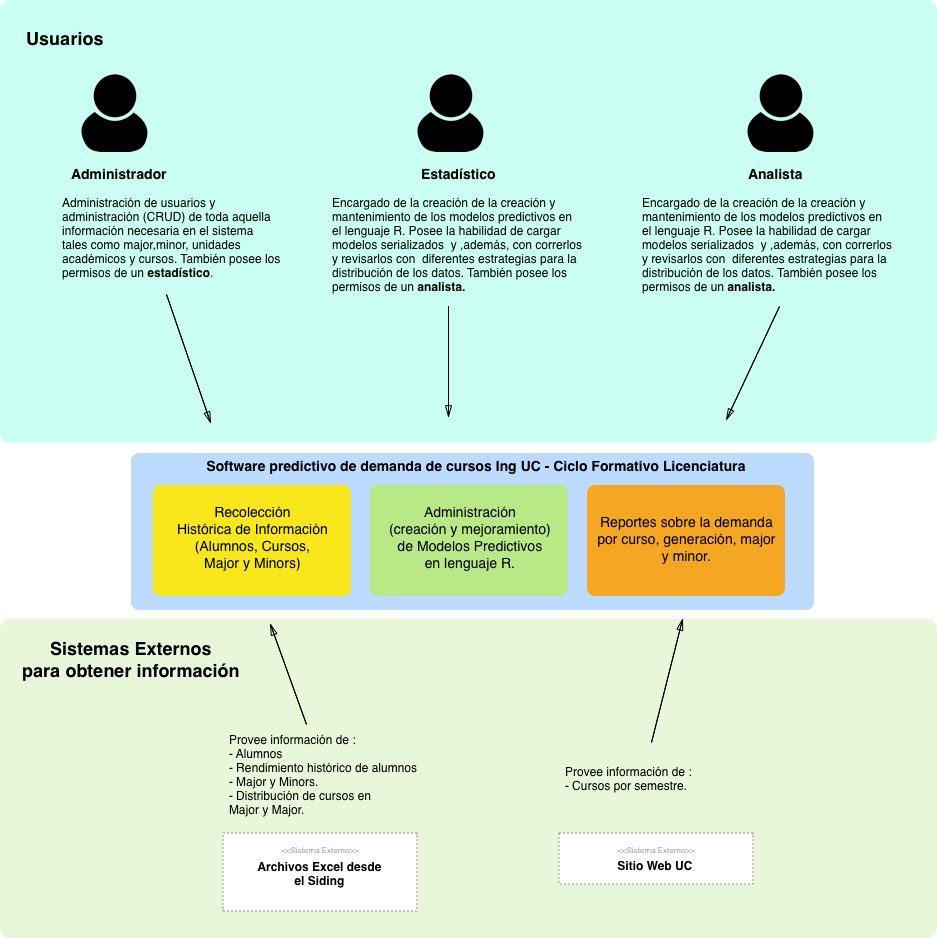
\includegraphics[width=0.95\textwidth]{./figures/chapter_03/02_diagrama_de_contexto.png}
		  \setcaptioncitation{Fuente Propia}
		  \caption{Diagrama de Contexto}
		  \label{fig:context_diagram_picture}
		\end{center}
	\end{figure}


\subsection{Diagrama de Componentes \label{sec:components_diagram}}

	\begin{figure}[H]
		\begin{center}
			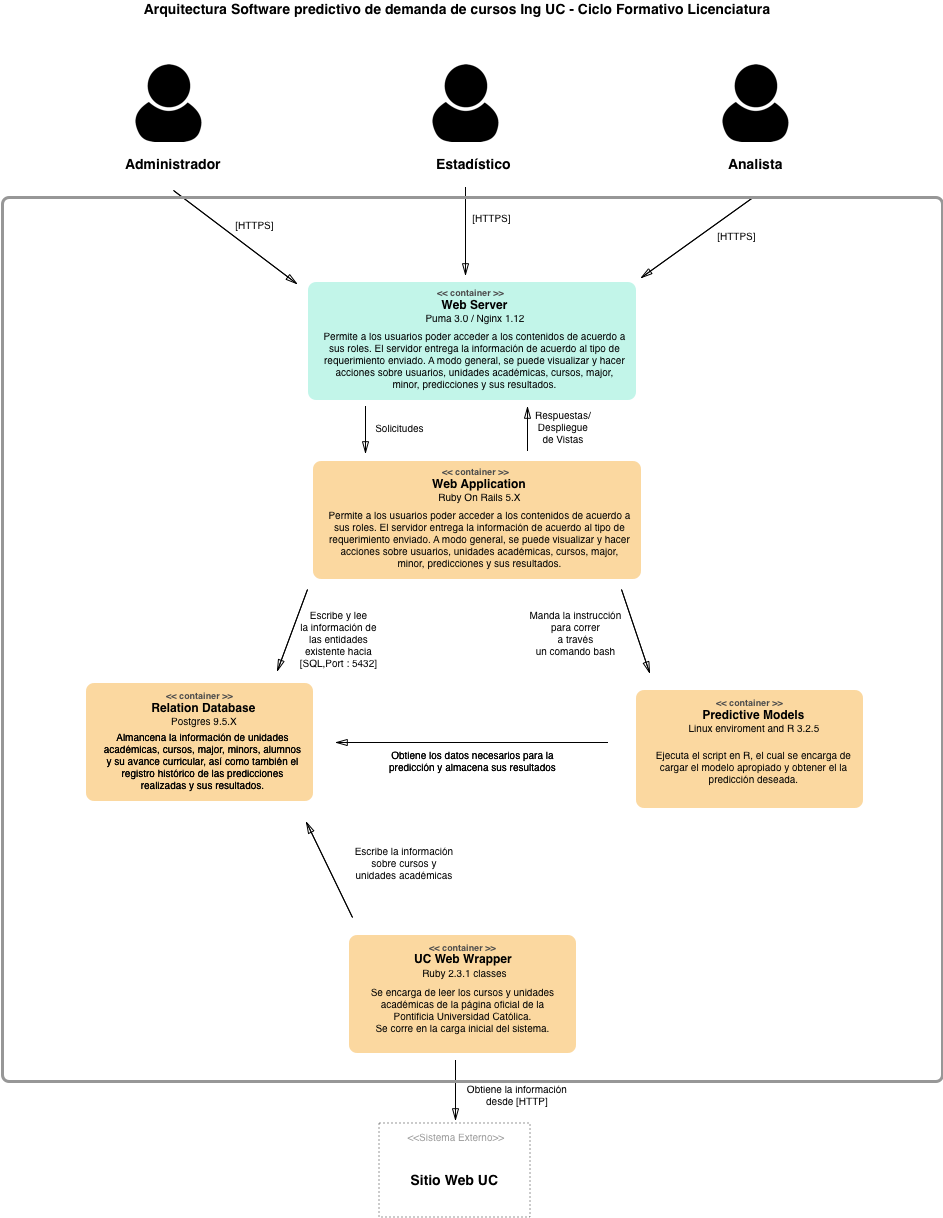
\includegraphics[width=0.9\textwidth]{./figures/chapter_03/03_diagrama_de_componentes.png}
			\setcaptioncitation{Fuente Propia}
			\caption{Diagrama de Componentes}
			\label{fig:components_diagram_picture}
		\end{center}
	\end{figure}


\subsection{Descripción de los Datos \label{sec:data_description}}

En las siguientes secciones se describen el conjunto datos y su estructura para realizar las predicciones de demanda de los cursos. En la primera parte se describe el modelo de base de datos utilizado y ,a continuación, el procedimiento de de cómo debe ir alimentándose el software para crear mantener la consistencia de la información.

\subsubsection{Modelo de datos \label{sec:data_model}}

El modelo de datos de la solución a implementar es el siguiente:

	\begin{figure}[H]
		\begin{center}
			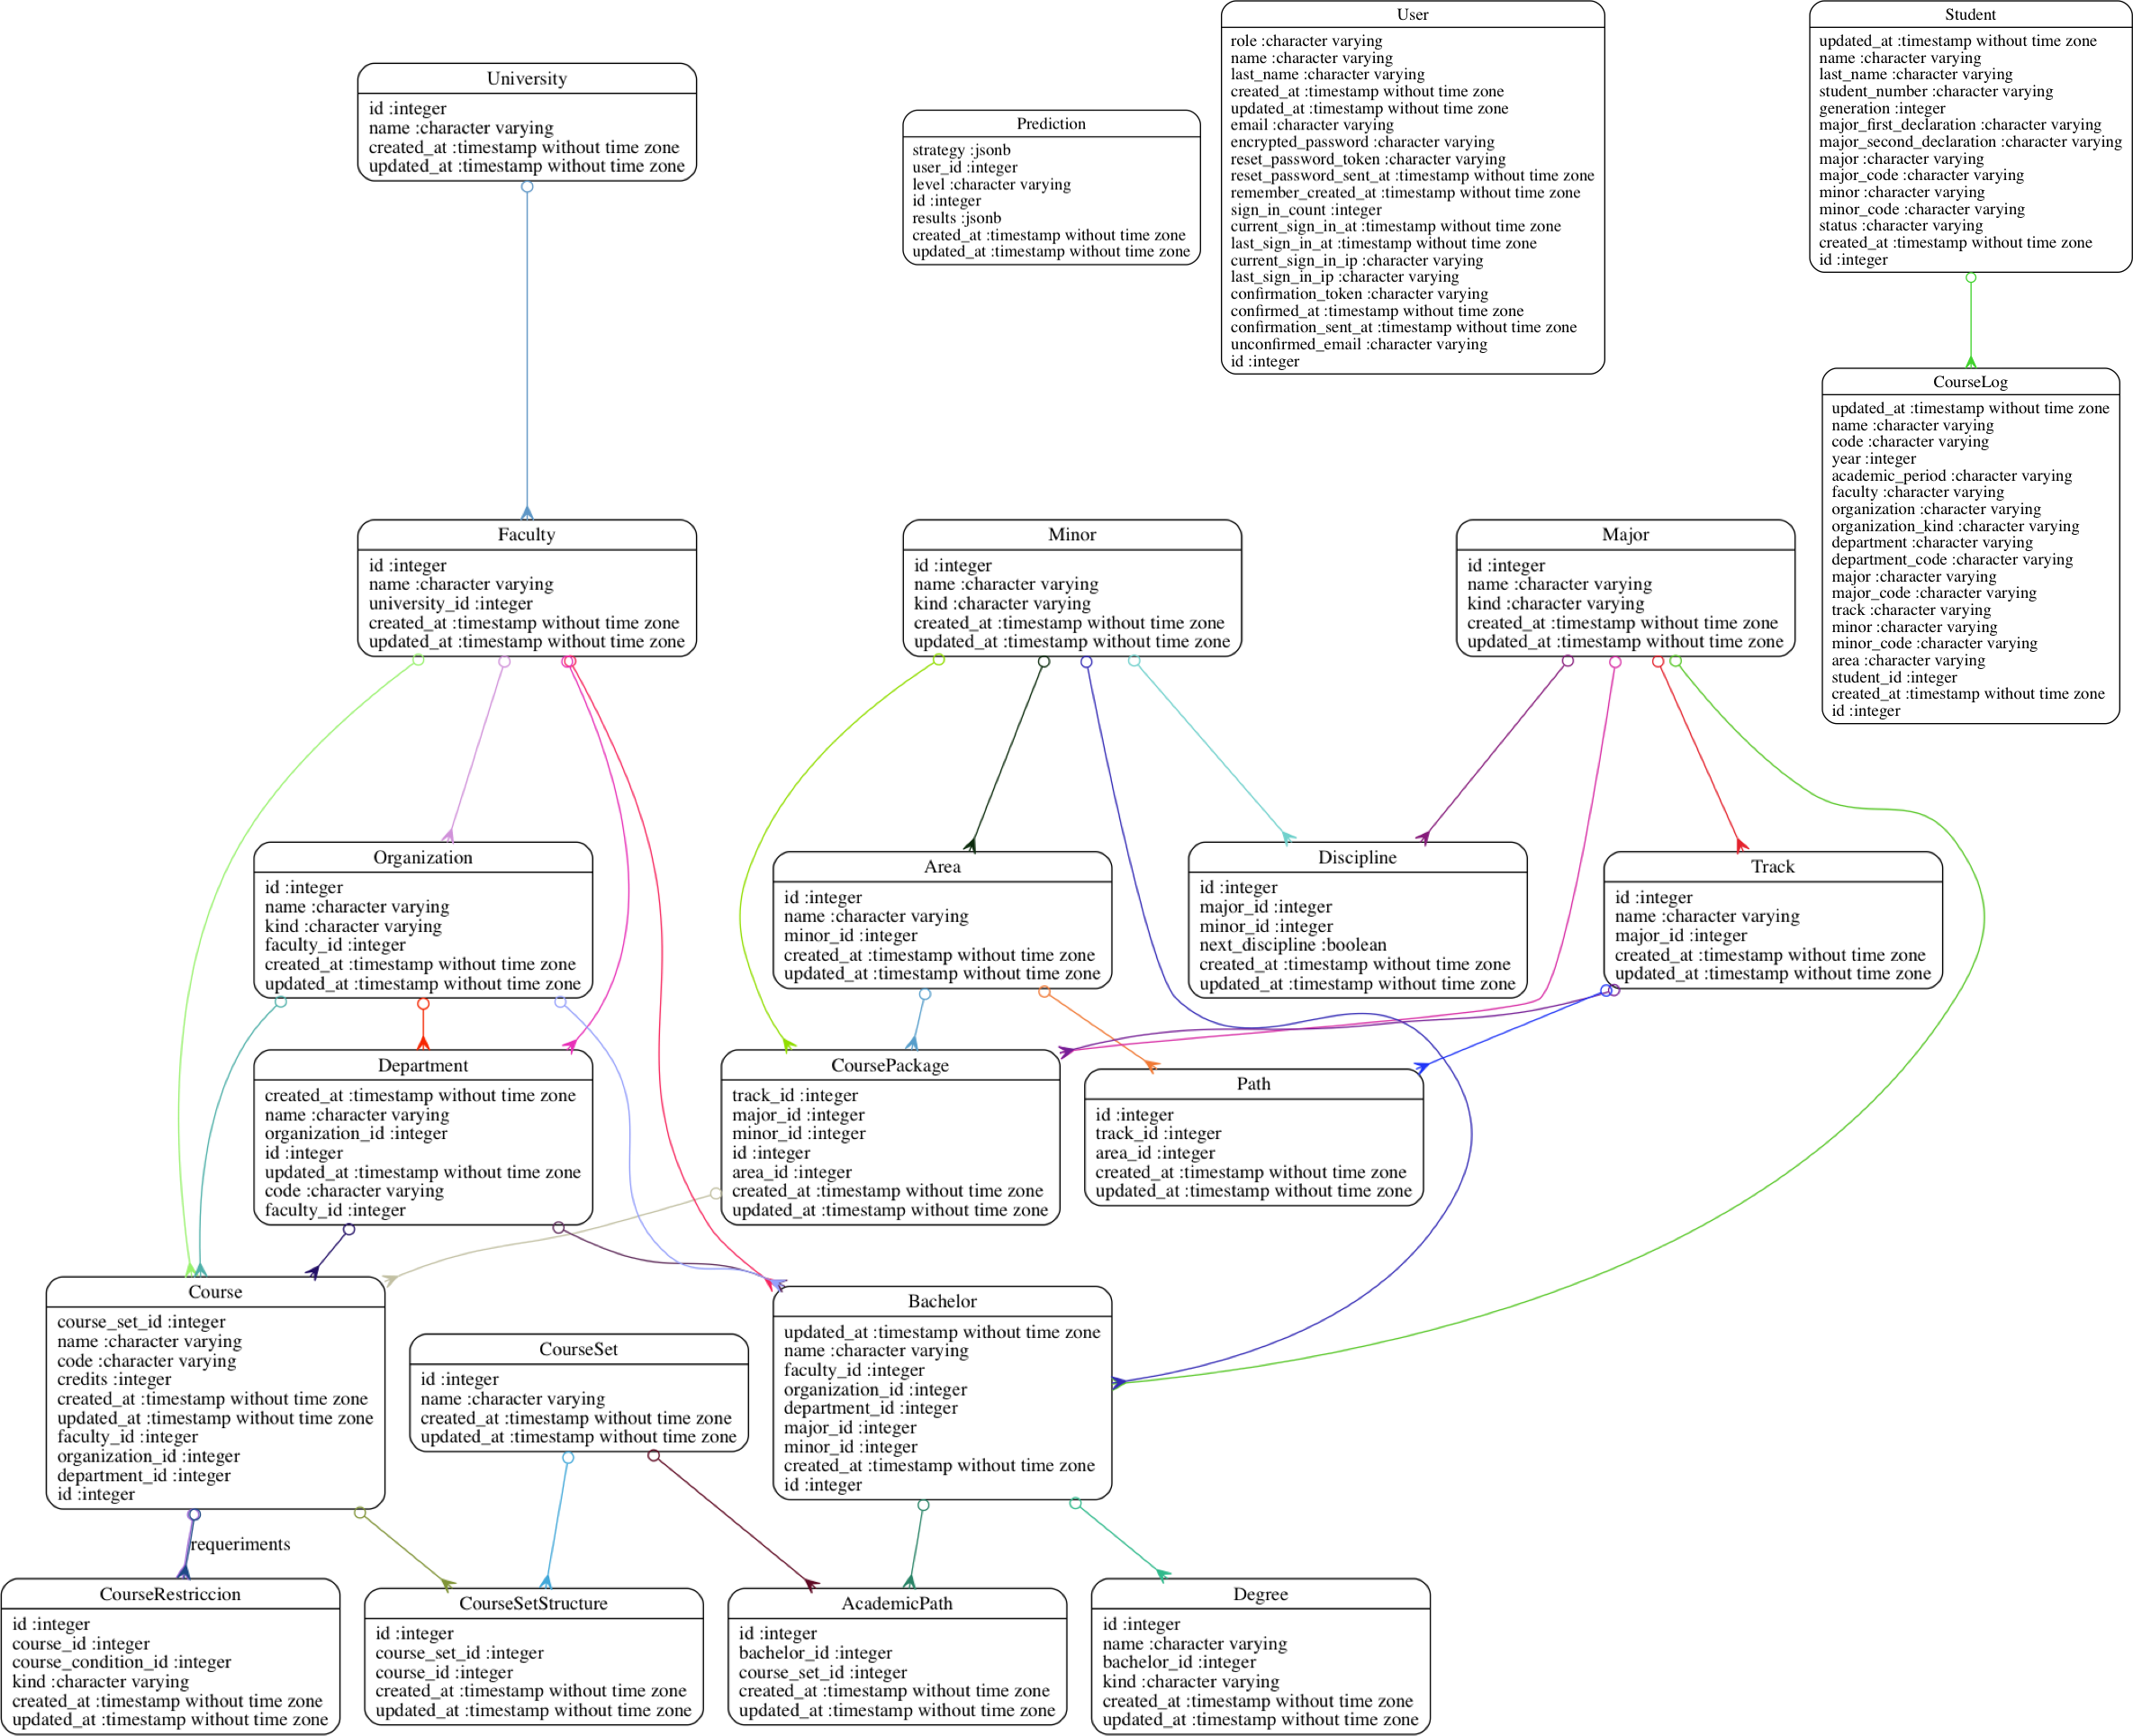
\includegraphics[width=0.95\textwidth]{./figures/chapter_03/04_modelo_de_datos.png}
			\setcaptioncitation{Fuente Propia}
			\caption{Modelo de Base de Datos}
			\label{fig:components_diagram_picture}
		\end{center}
	\end{figure}

Este modelo puede ser dividido de modo conceptual en las siguientes partes:

\begin{enumerate}
	\item \textbf{Universidad:} Las tablas \textit{University}, \textit{Faculty}, \textit{Organization}, \textit{Department}, \textit{Course} y CourseRestriccions permiten representar las relaciones entre la PUC, sus unidades académicas, los cursos que dictan y las requisitos que poseen.
	\item \textbf{Plan de Estudio:} El plan de estudio corresponde al conjunto de cursos que debe realizar un alumno para obtener un grado académico o título profesional UC. Las tablas que permiten almacenar esta información son: \textit{Bachelor}, \textit{Degree}, \textit{AcademicPath}, \textit{CourseSet}, \textit{CoureSetStructure}, \textit{Major}, \textit{Track}, \textit{Minor} y \textit{Area}. Además de las tablas intermedias descritas en el modelo de datos.
	\item \textbf{Predicciones de demanda:} Son las tablas que permiten llevar el registro de las predicciones solicitadas y sus resultados respectivamente. Las tablas que permiten esto son: \textit{Student}, \textit{CourseLog} y \textit{Predictions}. Cabe destacar que está última tabla posee un enfoque SQL y NoSQL debido a que posee dos columnas \textit{strategy} y \textit{results} en formato JSONB, el permite almacenar datos en formato JSON en representación binaria.
\end{enumerate}

El enfoque de diseño que se utilizó para el desarrollo de la base de datos fue modelo de Entidad Relación, para así permitir una mejor administración de unidades académicas, cursos y los alumnos dentro de la universidad en la plataforma. Con el fin de mantener las estadísticas y las predicciones de forma aislada , se crearon las tablas Student,CourseLog y Predictions.

\subsubsection{Carga Inicial \label{sec:initial_data_load}}

Dado que las proyecciones de demanda se basan en la información histórica del avance curricular de los alumnos se hace necesario poder cargar de forma inicial los elementos mencionados a continuación con el objetivo de poder realizar predicciones al momento de poner en marcha el sistema. Los elementos que cargan son los siguientes:

\begin{enumerate}
	\item \textbf{Universidad:} Nombre de universidad, facultades, centros de estudios (organization), escuelas (organization), departamentos, los cursos y sus requisitos o correquisitos de cursos.
	\item \textbf{Plan de Estudio:} Se hace la carga inicial de los major y sus tracks, minor y sus áreas, la relación entre ambos y los cursos pertenecientes a cada uno.
	\item \textbf{Avance Curricular:} Se hace carga del avance curricular de las generaciones del 2013 hacia adelante con la información actualizada hasta noviembre del 2016 entregada por Dirección de Pregrado.
\end{enumerate}

\subsubsection{Descripción de los Datos \label{sec:periodic_data_loads}}

Las cargas periódicas están enfocadas en mantener actualizada la información necesaria para las predicciones de demanda de cursos semestre a semestre, por lo tanto, se hace importante que el sistema cuenta con un sistema que permite realizar la carga de la siguiente información:

\begin{enumerate}
	\item \textbf{Información de Cursos:} Corresponde a la  carga masiva de cursos vigentes en la universidad, cabe destacar que el sistema no considera un curso en un periodo académico determinado, lo que busca es mantener actualizado sus cursos para determinar cuales son vigentes al momento de realizar una predicción.
	\item \textbf{Avance curricular de los alumnos:} Esta información es esencial para realizar predicciones más acertadas con el avance del tiempo.
\end{enumerate}

Ambas informaciones descritas anteriormente deben ser cargadas al finalizar un periodo académico, ya sea semestre o temporada académica de verano. El sistema posee un sistema de alerta que permite recordar a los usuarios administradores vía email y notificaciones en la plataforma web de que es necesario realizar este proceso. Debido a que cada año un semestre (primero o segundo) o temperada académica de verano inician y terminan en fechas diferentes, se crea una forma genérica para ir calculando un inicio y término ficticio, el cual es ajustable por un usuario administrador. Los criterios de cambio de periodo académico son los siguientes:

\begin{tabularx}{\linewidth}{@{}Y  Y  Y  Y@{}}
  \caption{Criterios de fechas para cambios de periodos académicos} \label{tab:university_structure}\\
  \toprule
  Periodo Académico	&	Fecha de Inicio Genérica	&	Fecha de Término Genérica
  \endhead
  \midrule
 	  Temporadad Académica de Verano (TAV) & 02 de Enero & 31 de Enero \\
  \midrule
  	Primer Semestre & 01 de Marzo & 15 de Julio \\
  \midrule
  	Segundo Semestre & 01 de Agosto & 15 de Diciembre \\
  \bottomrule
\end{tabularx}

Las fechas descritas anteriormente permiten al sistema cuán actualizada está su información con respecto al tiempo presente, se podrán efectuar predicciones siempre y cuando esta información esté actualizada al periodo académico anterior de cuando se desea realizar.
